\chapter{Real Business Cycles}

The preceding chapters focused on the \textbf{long-run} behavior of the economy: what determines the level and growth rate of output over decades. We now shift our attention to \textbf{short-run fluctuations}---the business cycle. The central question changes from ``Why do some countries grow faster than others?'' to ``Why does output fluctuate around its long-run trend, and what accounts for the patterns we observe in those fluctuations?''

\section{Defining the Business Cycle}

To study business cycles, we must first separate the data into what is ``trend'' and what is ``cycle.'' Consider the time series of log real GDP per capita, $y_t \equiv \ln(Y_t/\text{pop}_t)$. The raw data exhibits a clear upward trend (driven by long-run growth) with fluctuations around it. We decompose:
$$
y_t = y_t^T + y_t^C,
$$
where $y_t^T$ is the \textbf{trend component} and $y_t^C \equiv y_t - y_t^T$ is the \textbf{cyclical component} (the percentage deviation of output from trend).

\begin{center}
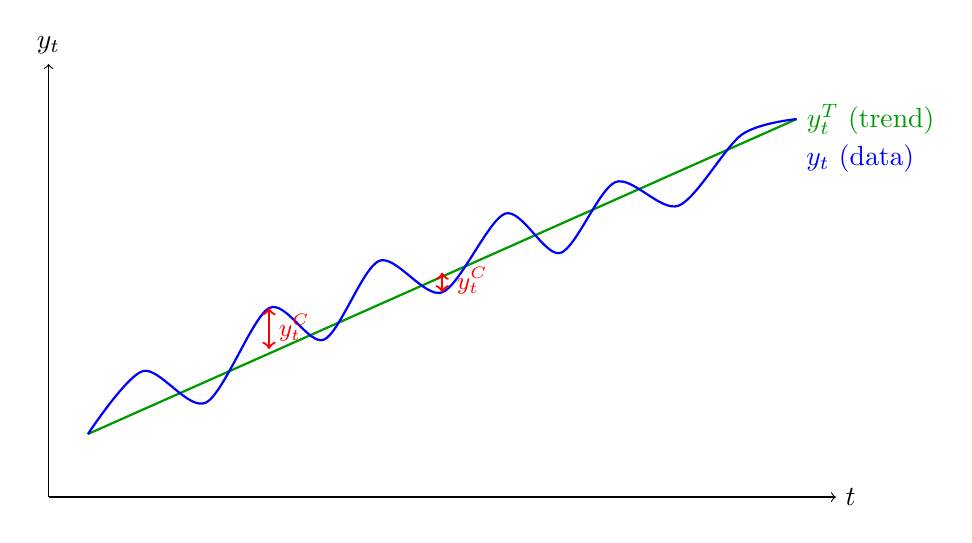
\begin{tikzpicture}[scale=1]
    \draw[->] (0,0) -- (10,0) node[right] {$t$};
    \draw[->] (0,0) -- (0,5.5) node[above] {$y_t$};
    % Trend
    \draw[thick, green!60!black] (0.5,0.8) -- (9.5,4.8) node[right] {$y_t^T$ (trend)};
    % Actual data (wavy line around trend)
    \draw[thick, blue] plot[smooth, tension=0.5] coordinates 
        {(0.5,0.8) (1.2,1.6) (2,1.2) (2.8,2.4) (3.5,2.0) (4.2,3.0) (5,2.6) (5.8,3.6) (6.5,3.1) (7.2,4.0) (8,3.7) (8.8,4.6) (9.5,4.8)};
    \node[blue, right] at (9.5,4.3) {$y_t$ (data)};
    % Cyclical component illustration
    \draw[<->, red, thick] (2.8,1.88) -- (2.8,2.4);
    \node[red, right] at (2.8,2.15) {\small $y_t^C$};
    \draw[<->, red, thick] (5,2.85) -- (5,2.6);
    \node[red, left] at (5.7,2.75) {\small $y_t^C$};
\end{tikzpicture}
\end{center}

\rmkb[The Trend-Cycle Decomposition is Not Unique]{
    The decomposition above is only as meaningful as the method used to extract the trend. Different detrending procedures---such as fitting a log-linear regression, the Hodrick-Prescott (HP) filter, or the Baxter-King band-pass filter---will produce different trend series $\{y_t^T\}_{t=0}^T$ and therefore different cyclical components $\{y_t^C\}_{t=0}^T$. The ``business cycle'' is not a directly observable object; it is defined by how we choose to remove the trend. This is an important caveat: empirical facts about business cycles are always conditional on the detrending method.
    \begin{center}
\begin{tikzpicture}[scale=1]
    \draw[->] (0,0) -- (10,0) node[right] {$t$};
    \draw[->] (0,0) -- (0,5.5) node[above] {$y_t$};
    % Actual data
    \draw[thick, blue] plot[smooth, tension=0.5] coordinates 
        {(0.5,0.5) (1.5,1.2) (2.5,1.0) (3.5,2.2) (4.5,1.8) (5.5,3.2) (6.5,2.8) (7.5,4.0) (8.5,3.5) (9.5,4.8)};
    \node[blue, above] at (9.5,4.8) {\small data};
    % Trend 1: linear
    \draw[thick, red, dashed] (0.5,0.6) -- (9.5,4.4) node[right] {\small linear trend};
    % Trend 2: flexible (HP filter style)
    \draw[thick, orange, densely dotted] plot[smooth, tension=0.6] coordinates 
        {(0.5,0.6) (1.5,1.0) (2.5,1.3) (3.5,1.8) (4.5,2.2) (5.5,2.8) (6.5,3.1) (7.5,3.6) (8.5,3.9) (9.5,4.5)};
    \node[orange, right] at (9.5,4.0) {\small HP trend};
\end{tikzpicture}
\end{center}
}

A \textbf{recession} is informally defined as two or more consecutive quarters in which \textit{real GDP falls relative to the previous quarter} (i.e., negative quarter-over-quarter growth), or equivalently, a sustained rise in the unemployment rate. This is a statement about the \textit{level} of GDP, not about its deviation from trend. In the United States, the official arbiter is the NBER Business Cycle Dating Committee, which considers a broader set of indicators---with particular weight on employment---rather than mechanically applying the two-quarter rule. Postwar U.S.\ recessions have averaged roughly 11 months in length, with a typical peak-to-trough decline of about 3\% in real GDP and a 2 percentage point increase in the unemployment rate.


\section{Three Key Facts about Business Cycles}

Any model that aspires to explain business cycles must be consistent with the following empirical regularities, documented extensively by King and Rebelo (1999):

\fact{Investment is more cyclical than output}{
    The cyclical component of investment has a much larger variance than that of output. More generally, the more durable a good is, the more cyclical its expenditure: housing and cars fluctuate far more than clothing or services. Nondurable consumption, by contrast, is \textit{less} cyclical than output (Bils, Klenow, and Malin, 2012).
}

\fact{Productivity (the Solow residual) is pro-cyclical}{
    Total factor productivity, measured as the Solow residual, comoves positively with output over the cycle. Output tends to be high when measured productivity is high, and vice versa.
}

\rmkb[The Solow Residual]{
    Given a Cobb-Douglas production function $Y_t = A_t K_t^\alpha L_t^{1-\alpha}$, the \textbf{Solow residual} is the component of output growth that cannot be accounted for by the growth of measured inputs:
    $$
    \ln A_t = \ln Y_t - \alpha \ln K_t - (1-\alpha) \ln L_t.
    $$
    It is often interpreted as a measure of total factor productivity (TFP). In practice, $\alpha$ is calibrated to the capital share of income (roughly 1/3 in the U.S.), and $K_t$, $L_t$, $Y_t$ are taken from national accounts data. The residual then captures everything that affects output beyond capital and labor---including technology, institutions, measurement error, and capacity utilization.
}

\fact{Total hours worked are about as cyclical as output}{
    Aggregate labor input fluctuates with roughly the same amplitude as output. Approximately 2/3 of the variation in total hours comes from the \textit{extensive margin} (the number of employed workers), and 1/3 from the \textit{intensive margin} (hours per worker).
}

\section{Why the Solow Model Fails as a Business Cycle Model}

A natural first attempt is to use the Solow model we already know as a theory of fluctuations. Suppose TFP $A_t$ fluctuates around a constant level $A^*$---say, $A_t \in \{A^* e^{\ve}, A^* e^{-\ve}\}$ for some small $\ve > 0$. In the Solow diagram, this shifts the saving curve $s A_t f(k_t)$ up and down, causing the steady-state capital stock to oscillate between two values. The economy would indeed exhibit cyclical behavior in $k_t$ and $y_t$.

\begin{center}
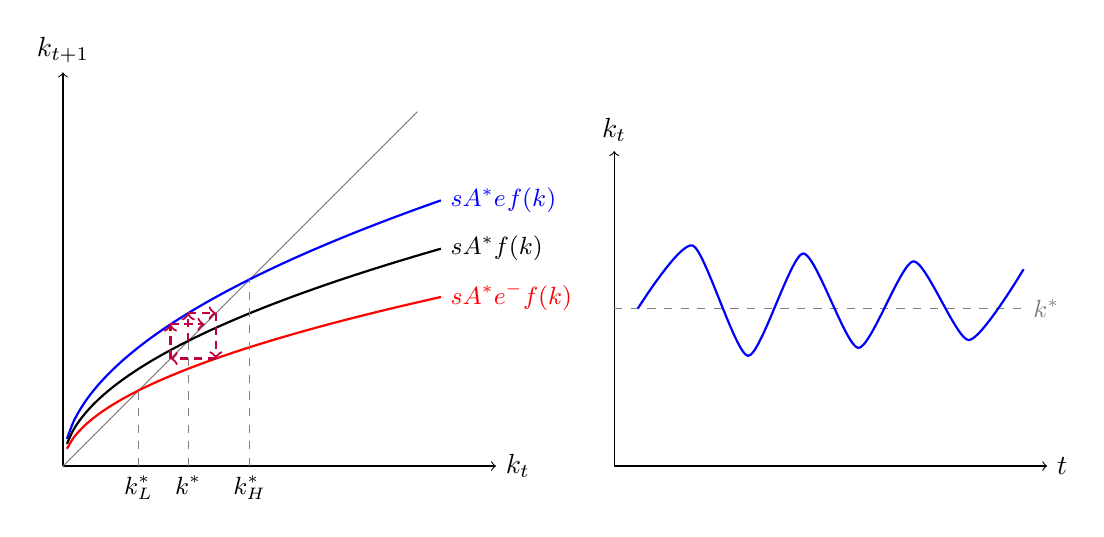
\begin{tikzpicture}[scale=1]
    % Left panel: Solow diagram
    \draw[->] (0,0) -- (5.5,0) node[right] {$k_t$};
    \draw[->] (0,0) -- (0,5) node[above] {$k_{t+1}$};
    % 45-degree line
    \draw[gray, thin] (0,0) -- (4.5,4.5);
    
    % Curves: k_{t+1} = sAf(k) + (1-delta)k, simplified as concave curves
    % Blue (high A): 1.54*sqrt(x), crosses 45 at x ≈ 2.37
    \draw[thick, blue] plot[smooth, domain=0.05:4.8, samples=60] (\x, {1.54*sqrt(\x)});
    % Black (middle A): 1.26*sqrt(x), crosses 45 at x ≈ 1.59
    \draw[thick, black] plot[smooth, domain=0.05:4.8, samples=60] (\x, {1.26*sqrt(\x)});
    % Red (low A): 0.98*sqrt(x), crosses 45 at x ≈ 0.96
    \draw[thick, red] plot[smooth, domain=0.05:4.8, samples=60] (\x, {0.98*sqrt(\x)});
    
    % Labels: placed at the right end of each curve, stacked clearly
    \node[blue, right] at (4.8,{1.54*sqrt(4.8)}) {\small $sA^*e^{\ve}f(k)$};
    \node[black, right] at (4.8,{1.26*sqrt(4.8)}) {\small $sA^*f(k)$};
    \node[red, right] at (4.8,{0.98*sqrt(4.8)}) {\small $sA^*e^{-\ve}f(k)$};
    
    % Steady state markers
    \draw[dashed, gray] (2.37,0) -- (2.37,2.37);
    \node[below, font=\small] at (2.37,0) {$k_H^*$};
    \draw[dashed, gray] (1.59,0) -- (1.59,1.59);
    \node[below, font=\small] at (1.59,0) {$k^*$};
    \draw[dashed, gray] (0.96,0) -- (0.96,0.96);
    \node[below, font=\small] at (0.96,0) {$k_L^*$};
    
    % Dynamics: start at k*=1.59, alternate high/low A
    % Period 0: k0 = 1.59, A high -> k1 = 1.54*sqrt(1.59) ≈ 1.94
    \draw[->, thick, purple, densely dashed] (1.59,1.59) -- (1.59,{1.54*sqrt(1.59)});
    \draw[->, thick, purple, densely dashed] (1.59,{1.54*sqrt(1.59)}) -- ({1.54*sqrt(1.59)},{1.54*sqrt(1.59)});
    % Period 1: k1 = 1.94, A low -> k2 = 0.98*sqrt(1.94) ≈ 1.36
    \draw[->, thick, purple, densely dashed] ({1.54*sqrt(1.59)},{1.54*sqrt(1.59)}) -- ({1.54*sqrt(1.59)},{0.98*sqrt(1.54*sqrt(1.59))});
    \draw[->, thick, purple, densely dashed] ({1.54*sqrt(1.59)},{0.98*sqrt(1.54*sqrt(1.59))}) -- ({0.98*sqrt(1.54*sqrt(1.59))},{0.98*sqrt(1.54*sqrt(1.59))});
    % Period 2: k2 ≈ 1.36, A high -> k3 = 1.54*sqrt(1.36) ≈ 1.80
    \draw[->, thick, purple, densely dashed] ({0.98*sqrt(1.94)},{0.98*sqrt(1.94)}) -- ({0.98*sqrt(1.94)},{1.54*sqrt(0.98*sqrt(1.94))});
    \draw[->, thick, purple, densely dashed] ({0.98*sqrt(1.94)},{1.54*sqrt(0.98*sqrt(1.94))}) -- ({1.54*sqrt(0.98*sqrt(1.94))},{1.54*sqrt(0.98*sqrt(1.94))});
    
    % Right panel: k_t over time
    \begin{scope}[xshift=7cm]
        \draw[->] (0,0) -- (5.5,0) node[right] {$t$};
        \draw[->] (0,0) -- (0,4) node[above] {$k_t$};
        \draw[dashed, gray] (0,2) -- (5.2,2) node[right] {\small $k^*$};
        \draw[thick, blue] plot[smooth, tension=0.4] coordinates 
            {(0.3,2) (1,2.8) (1.7,1.4) (2.4,2.7) (3.1,1.5) (3.8,2.6) (4.5,1.6) (5.2,2.5)};
    \end{scope}
\end{tikzpicture}
\end{center}

However, the Solow model imposes a \textbf{constant saving rate}: $I_t = s Y_t$. This immediately implies
$$
\ln I_t = \ln s + \ln Y_t.
$$
Taking variances of both sides:
$$
\Var{\ln I_t} = \Var{\ln Y_t} + \underbrace{\Var{\ln s}}_{= 0},
$$
so $\Var{\ln I_t} = \Var{\ln Y_t}$. That is, investment is \textit{exactly as cyclical} as output.

\rmkb[]{
This directly contradicts \textbf{Fact 1}. In the data, the variance of cyclical investment is several times larger than that of cyclical output. The source of the failure is clear: the Solow model treats the saving rate as an exogenous constant, so agents cannot choose to save more in booms and less in recessions. To generate excess volatility of investment, we need a model in which the saving (equivalently, consumption-investment) decision is made optimally by forward-looking agents. This is the motivation for the \textbf{Real Business Cycle (RBC)} model, which replaces the mechanical saving rule with a fully microfounded dynamic optimization problem.
}

\section{An RBC Model with Fixed Labor}

Having established that the Solow model fails to match the key business cycle facts due to its constant saving rate, we now build a model in which the consumption-saving decision is made optimally by a forward-looking planner. This is the \textbf{Real Business Cycle (RBC)} model, originating from Kydland and Prescott (1982). In this simplified version, we fix labor supply and focus on how stochastic productivity shocks, combined with optimal intertemporal choice, generate cyclical fluctuations that are qualitatively consistent with the data.

\subsection{Environment}

\begin{itemize}
    \item \textbf{Time:} Discrete, $t = 0, 1, 2, \ldots$
    \item \textbf{Preferences:} A representative planner maximizes expected discounted lifetime utility:
    $$
    U\left(\{c_t\}_{t=0}^\infty\right) = \E{\sum_{t=0}^{\infty} \beta^t u(c_t)},
    $$
    where $\beta \in (0,1)$ is the discount factor and $u(\cdot)$ is a strictly concave, increasing period utility function.
    \item \textbf{Production:} The aggregate production function exhibits constant returns to scale: $Y_t = A_t F(K_t, L)$. Since labor $L$ is fixed (normalized to 1), we can write everything in per-capita terms. Define $k_t \equiv K_t / L$ and $f(k_t) \equiv F(K_t/L,\, L/L) = F(k_t, 1)$. Then output per capita is:
    $$
    y_t = e^{a_t} f(k_t),
    $$
    where $a_t \equiv \ln A_t$ is log-TFP. The stochastic process $\{a_t\}$ is the sole source of randomness in the model.
    \item \textbf{Stochastic Process for Technology:} The log-TFP process $\{a_t\}_{t=0}^\infty$ follows a \textbf{Markov process} with a time-invariant conditional distribution $\pi(a_{t+1} \mid a_t)$. 
    
    \item \textbf{Resource Constraint:} In every period,
    $$
    c_t + k_{t+1} = e^{a_t} f(k_t) + (1-\delta) k_t, \quad \forall\, t \geq 0,
    $$
    where $\delta \in (0,1)$ is the depreciation rate.
\end{itemize}

\rmkb[Timing and Information]{
    The timing within each period is as follows. At the beginning of period $t$, the planner enters with capital $k_t$ (chosen last period) and observes the realization of $a_t$, drawn from $\pi(a_t \mid a_{t-1})$. After observing $a_t$, the planner chooses consumption $c_t$ and next-period capital $k_{t+1}$. Then at $t+1$, the new shock $a_{t+1}$ is realized, and the process repeats.
    
    Crucially, the planner's decision at time $t$ can depend on the \textit{current} state $(a_t, k_t)$ but not on future realizations of $a$. This is why we look for a policy function of the form $k_{t+1} = g(a_t, k_t)$.

    \begin{center}
    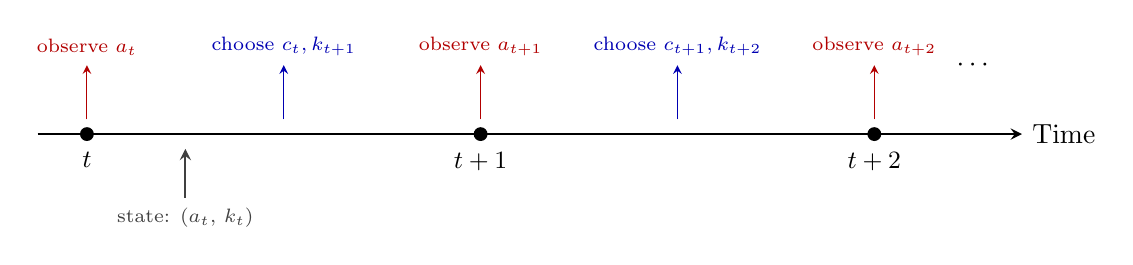
\begin{tikzpicture}[scale=1.25, >=stealth]
        % Timeline
        \draw[thick, ->] (0,0) -- (10,0) node[right] {Time};
        % Period markers
        \foreach \x/\lab in {0.5/t, 4.5/{t+1}, 8.5/{t+2}} {
            \fill (\x, 0) circle (2pt);
            \node[below=3pt, font=\small] at (\x, 0) {$\lab$};
        }
        % Events above the line (observe) and below the line (choose)
        % Period t
        \draw[->, red!70!black] (0.5, 0.15) -- (0.5, 0.7);
        \node[above, align=center, font=\scriptsize, red!70!black] at (0.5, 0.7) {observe $a_t$};
        \draw[->, blue!70!black] (2.5, 0.15) -- (2.5, 0.7);
        \node[above, align=center, font=\scriptsize, blue!70!black] at (2.5, 0.7) {choose $c_t, k_{t+1}$};
        % Period t+1
        \draw[->, red!70!black] (4.5, 0.15) -- (4.5, 0.7);
        \node[above, align=center, font=\scriptsize, red!70!black] at (4.5, 0.7) {observe $a_{t+1}$};
        \draw[->, blue!70!black] (6.5, 0.15) -- (6.5, 0.7);
        \node[above, align=center, font=\scriptsize, blue!70!black] at (6.5, 0.7) {choose $c_{t+1}, k_{t+2}$};
        % Period t+2
        \draw[->, red!70!black] (8.5, 0.15) -- (8.5, 0.7);
        \node[above, align=center, font=\scriptsize, red!70!black] at (8.5, 0.7) {observe $a_{t+2}$};
        \node at (9.5, 0.7) {$\cdots$};
        % State annotation: arrow pointing to the interval
        \draw[<-, thick, darkgray] (1.5, -0.15) -- (1.5, -0.65);
        \node[below, font=\scriptsize, darkgray] at (1.5, -0.65) {state: $(a_t,\, k_t)$};
    \end{tikzpicture}
    \end{center}
}

\subsection{The Planner's Problem}

By the principle of optimality, the planner's problem can be written recursively. The \textbf{value function} $V(a, k)$ satisfies the Bellman equation:
$$
\begin{aligned}
    V(a, k) & =  \max_{\substack{c > 0 \\ k' \geq 0}} \left\{ u(c) + \beta\, \E{V(a', k') \mid a} \right\}\\
\text{s.t.} &  \quad c + k' = e^a f(k) + (1-\delta) k.
\end{aligned}
$$

\noindent The associated \textbf{policy function} is:
$$
g(a, k) = \argmax_{\substack{c > 0 \\ k' \geq 0}} \left\{ u(c) + \beta\, \E{V(a', k') \mid a} \right\} \quad \text{s.t.} \quad c + k' = e^a f(k) + (1-\delta) k.
$$

Unlike the deterministic Solow model, the saving rate here is \textit{endogenous}: the planner optimally chooses how much to consume and how much to invest, conditional on the current state of technology. When productivity is temporarily high, the planner may choose to save a larger fraction of output (investing for the future), and when productivity is low, the planner may dissave. This endogenous response is precisely what allows the model to generate investment volatility in excess of output volatility.

\subsection{Numerical Solution by Value Function Iteration}

To solve the model concretely, consider a tractable special case in which technology takes only two values:
$$
a_t \in \{a_H, a_L\}, \quad a_H > a_L,
$$
with transitions governed by a $2 \times 2$ Markov transition matrix:
$$
\Pi = \begin{pmatrix} \pi_{HH} & \pi_{HL} \\ \pi_{LH} & \pi_{LL} \end{pmatrix},
$$
where $\pi_{ij} = \Pr{a_{t+1} = a_j \mid a_t = a_i}$ and each row sums to 1.

\rmkb[]{
    Persistence in the productivity process (i.e., $\pi_{HH}$ and $\pi_{LL}$ being large) is important for generating realistic business cycles. If shocks were purely i.i.d., the economy would revert to its mean too quickly, producing cycles that are too short and too shallow relative to the data.
}

The Bellman equation generally does not admit a closed-form solution, so we solve it numerically. The key idea is to \textbf{discretize} the capital state space and iterate on the value function until convergence.

To begin with, we discretize the capital space into a grid of $N$ points:
$$
\mathcal{K} = \{k^1, k^2, \ldots, k^N\}.
$$

The objects we seek are:
\begin{itemize}
    \item \textbf{Value function:} An $N \times 2$ matrix $\mathbf{V} = [\mathbf{V}_H, \mathbf{V}_L]$, where $V_H^n \equiv V(a_H, k^n)$ and $V_L^n \equiv V(a_L, k^n)$.
    \item \textbf{Policy function:} An $N \times 2$ matrix $\mathbf{g} = [\mathbf{g}_H, \mathbf{g}_L]$, where $g_H^n \equiv g(a_H, k^n)$ and $g_L^n \equiv g(a_L, k^n)$.
\end{itemize}

\begin{center}
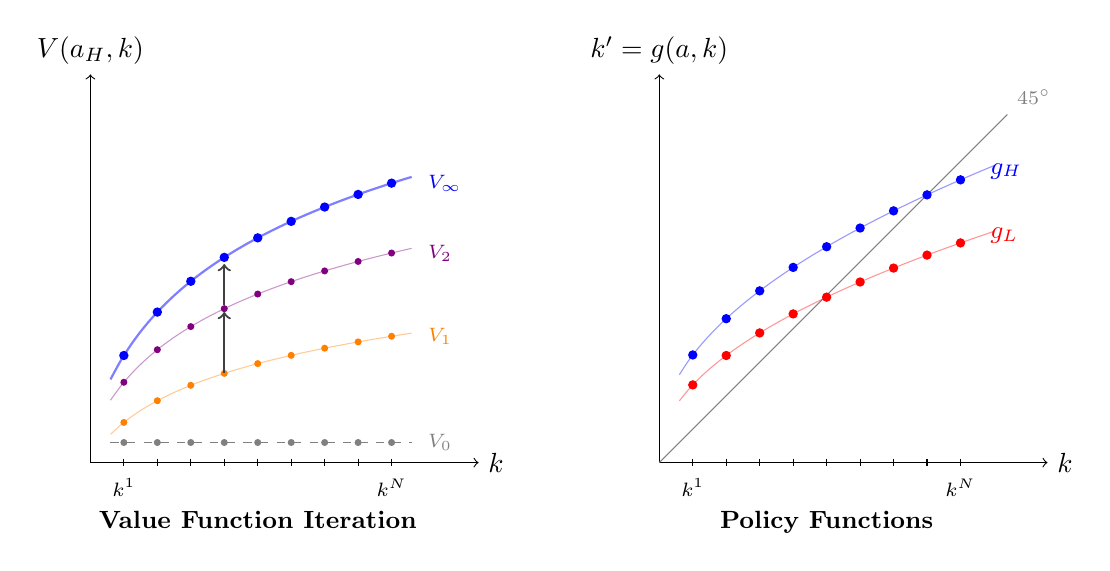
\begin{tikzpicture}[scale=0.85]
    \draw[->] (0,0) -- (5.8,0) node[right] {$k$};
        \draw[->] (0,0) -- (0,5.8) node[above] {$V(a_H,k)$};
        % V_0 (flat at 0)
        \draw[gray, dashed, thin] (0.3,0.3) -- (4.8,0.3);
        \foreach \k in {0.5, 1.0, 1.5, 2.0, 2.5, 3.0, 3.5, 4.0, 4.5} {
            \fill[gray] (\k, 0.3) circle (1.5pt);
        }
        \node[gray, right, font=\scriptsize] at (4.9, 0.3) {$V_0$};
        % V_1 (slightly concave)
        \draw[orange, thin, opacity=0.4] plot[smooth, domain=0.3:4.8, samples=30] (\x, {0.6+0.8*ln(\x+0.5)});
        \foreach \k in {0.5, 1.0, 1.5, 2.0, 2.5, 3.0, 3.5, 4.0, 4.5} {
            \fill[orange] (\k, {0.6+0.8*ln(\k+0.5)}) circle (1.5pt);
        }
        \node[orange, right, font=\scriptsize] at (4.9, {0.6+0.8*ln(5)}) {$V_1$};
        % V_2 (more concave)
        \draw[violet, thin, opacity=0.4] plot[smooth, domain=0.3:4.8, samples=30] (\x, {1.2+1.2*ln(\x+0.5)});
        \foreach \k in {0.5, 1.0, 1.5, 2.0, 2.5, 3.0, 3.5, 4.0, 4.5} {
            \fill[violet] (\k, {1.2+1.2*ln(\k+0.5)}) circle (1.5pt);
        }
        \node[violet, right, font=\scriptsize] at (4.9, {1.2+1.2*ln(5)}) {$V_2$};
        % V_infty (converged)
        \draw[blue, thick, opacity=0.5] plot[smooth, domain=0.3:4.8, samples=30] (\x, {1.6+1.6*ln(\x+0.5)});
        \foreach \k in {0.5, 1.0, 1.5, 2.0, 2.5, 3.0, 3.5, 4.0, 4.5} {
            \fill[blue] (\k, {1.6+1.6*ln(\k+0.5)}) circle (2pt);
        }
        \node[blue, right, font=\scriptsize] at (4.9, {1.6+1.6*ln(5)}) {$V_\infty$};
        % Arrow indicating iteration direction
        \draw[->, thick, darkgray] (2, {0.6+0.8*ln(2.5)}) -- (2, {1.15+1.2*ln(2.5)});
        \draw[->, thick, darkgray] (2, {1.25+1.2*ln(2.5)}) -- (2, {1.5+1.6*ln(2.5)});
        % Grid ticks
        \foreach \k in {0.5, 1.0, 1.5, 2.0, 2.5, 3.0, 3.5, 4.0, 4.5} {
            \draw (\k, 1.5pt) -- (\k, -1.5pt);
        }
        \node[below, font=\scriptsize] at (0.5, -0.1) {$k^1$};
        \node[below, font=\scriptsize] at (4.5, -0.1) {$k^N$};
        \node[below=14pt, font=\small] at (2.5, 0) {\textbf{Value Function Iteration}};
    
    % ---- Right panel: Value function iteration ----
    \begin{scope}[xshift=8.5cm]
        % ---- Left panel: Policy functions ----
    \draw[->] (0,0) -- (5.8,0) node[right] {$k$};
    \draw[->] (0,0) -- (0,5.8) node[above] {$k'=g(a,k)$};
    \draw[gray, thin] (0,0) -- (5.2,5.2) node[above right, font=\scriptsize, gray] {$45^\circ$};
    % g_H curve and dots
    \draw[blue, thin, opacity=0.4] plot[smooth, domain=0.3:5, samples=40] (\x, {0.3+1.85*sqrt(\x)});
    \foreach \k in {0.5, 1.0, 1.5, 2.0, 2.5, 3.0, 3.5, 4.0, 4.5} {
        \fill[blue] (\k, {0.3+1.85*sqrt(\k)}) circle (2pt);
    }
    \node[blue, right, font=\small] at (4.8, {0.3+1.85*sqrt(4.8)}) {$g_H$};
    % g_L curve and dots
    \draw[red, thin, opacity=0.4] plot[smooth, domain=0.3:5, samples=40] (\x, {0.1+1.5*sqrt(\x)});
    \foreach \k in {0.5, 1.0, 1.5, 2.0, 2.5, 3.0, 3.5, 4.0, 4.5} {
        \fill[red] (\k, {0.1+1.5*sqrt(\k)}) circle (2pt);
    }
    \node[red, right, font=\small] at (4.8, {0.1+1.5*sqrt(4.8)}) {$g_L$};
    % Grid ticks on x-axis
    \foreach \k in {0.5, 1.0, 1.5, 2.0, 2.5, 3.0, 3.5, 4.0, 4.5} {
        \draw (\k, 1.5pt) -- (\k, -1.5pt);
    }
    \node[below, font=\scriptsize] at (0.5, -0.1) {$k^1$};
    \node[below, font=\scriptsize] at (4.5, -0.1) {$k^N$};
    \node[below=14pt, font=\small] at (2.5, 0) {\textbf{Policy Functions}};
    \end{scope}
\end{tikzpicture}
\end{center}

\state{Value Function Iteration Algorithm for the RBC Model}{
    \begin{enumerate}[label=\textbf{Step \arabic*:}, leftmargin=*]
    \item \textbf{Initialize.} Guess an initial value function $\mathbf{V}_0 = [\mathbf{V}_{H,0},\, \mathbf{V}_{L,0}]$. A natural starting point is $\mathbf{V}_0 = \mathbf{0}$ (the $N \times 2$ zero matrix). Set the iteration counter $\texttt{nI} = 0$.
    
    \item \textbf{Update.} For each grid point $k^n$ and each technology state, compute the updated value by solving a finite maximization problem. For the high state:
    $$
    V_{H,\texttt{nI}+1}^n = \max_{n' \in \{1, \ldots, N\}} \left\{ u\!\left[e^{a_H} f(k^n) + (1-\delta)k^n - k^{n'}\right] + \beta\!\left(\pi_{HH}\, V_{H,\texttt{nI}}^{n'} + \pi_{HL}\, V_{L,\texttt{nI}}^{n'}\right) \right\},
    $$
    and analogously for the low state:
    $$
    V_{L,\texttt{nI}+1}^n = \max_{n' \in \{1, \ldots, N\}} \left\{ u\!\left[e^{a_L} f(k^n) + (1-\delta)k^n - k^{n'}\right] + \beta\!\left(\pi_{LH}\, V_{H,\texttt{nI}}^{n'} + \pi_{LL}\, V_{L,\texttt{nI}}^{n'}\right) \right\}.
    $$
    Record the optimizer $n'_H(n)$ and $n'_L(n)$ at each grid point. Set $\texttt{nI} \leftarrow \texttt{nI} + 1$.
    
    \item \textbf{Check convergence.} If $\|\mathbf{V}_{\texttt{nI}} - \mathbf{V}_{\texttt{nI}-1}\| < \varepsilon$ for a small tolerance $\varepsilon > 0$, stop. Otherwise, return to Step 2.
    
    \item \textbf{Extract the policy function.} Using the optimizers from the final iteration, construct:
    $$
    g_H^n = k^{n_H^*(n)}, \qquad g_L^n = k^{n_L^*(n)}, \qquad \text{for } n = 1, \ldots, N.
    $$
\end{enumerate}
}

\rmkb[Properties of the Solution]{
    The converged solution has two intuitive properties:
    \begin{itemize}
        \item \textbf{Policy functions:} $g_H(k) > g_L(k)$ for all $k$---when productivity is high, the planner invests more (chooses higher $k'$). Both policy functions lie below the 45-degree line for large $k$ (capital eventually decays if no new investment is made) and above it for small $k$.
        \item \textbf{Value functions:} $V_H(k) > V_L(k)$ for all $k$---the planner is strictly better off when productivity is high, holding capital fixed. Both are increasing and concave in $k$.
    \end{itemize}
}

\subsection{Simulation and Evaluating the Model}

With the policy function in hand, we can simulate the model economy and check whether it reproduces the key business cycle facts.

\begin{enumerate}[label=\textbf{Step \arabic*:}, leftmargin=*]
    \item \textbf{Draw shocks.} Simulate a sequence $\{a_t\}_{t=0}^{T}$ (e.g., $T = 100$) from the Markov chain $\Pi$.
    
    \item \textbf{Generate capital path.} Starting from an initial $k_0$, iterate forward using the policy function:
    $$
    k_{t+1} = g(a_t, k_t), \quad t = 0, 1, \ldots, T.
    $$
    
    \item \textbf{Recover all variables.} For each $t$:
    $$
    y_t = e^{a_t} f(k_t), \qquad I_t = k_{t+1} - (1-\delta)k_t, \qquad c_t = y_t - I_t.
    $$
    
    \item \textbf{Compute business cycle statistics.} To compare the cyclicality of variables that differ in scale (output is much larger than investment in levels), we use the \textbf{coefficient of variation}---the standard deviation divided by the mean:
    $$
    \text{CV}(x_t) \equiv \frac{\sqrt{\Var{x_t}}}{\bar{x}} = \sqrt{\Var{\frac{x_t}{\bar{x}}}}.
    $$
    This is a unit-free measure of volatility: it tells us the \textit{percentage} fluctuation of a variable around its mean. For instance, $\text{CV}(I_t) = 0.10$ means investment fluctuates by roughly $\pm 10\%$ around its average level.
    
    The RBC model predicts:
    $$
    \text{CV}(I_t) > \text{CV}(y_t) > \text{CV}(c_t),
    $$
    i.e., \textbf{investment is more volatile than output, and consumption is smoother than output}.

    \begin{center}
    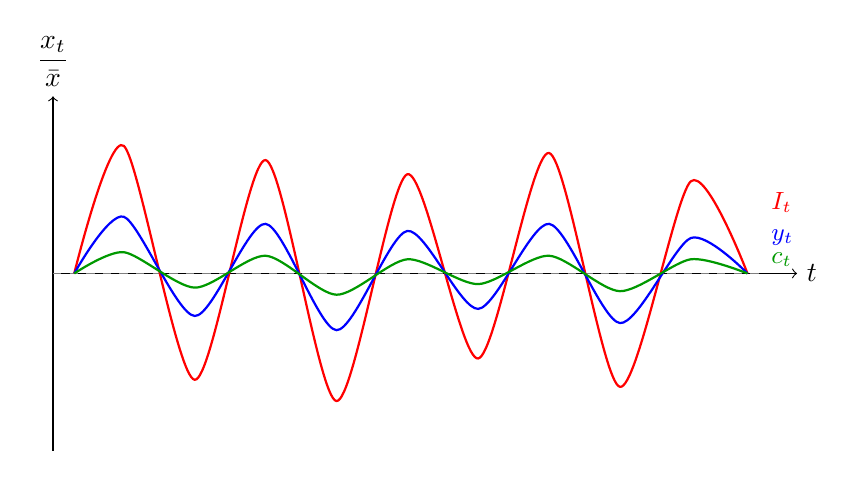
\begin{tikzpicture}[scale=0.9]
        \draw[->] (0,0) -- (10.5,0) node[right] {$t$};
        \draw[->] (0,-2.5) -- (0,2.5) node[above] {$\displaystyle\frac{x_t}{\bar{x}}$};
        \draw[gray, dashed] (0,0) -- (10,0);
        % Investment: high amplitude
        \draw[thick, red] plot[smooth, tension=0.45] coordinates 
            {(0.3,0) (1,1.8) (2,-1.5) (3,1.6) (4,-1.8) (5,1.4) (6,-1.2) (7,1.7) (8,-1.6) (9,1.3) (9.8,0)};
        \node[red, right, font=\small] at (10, 1) {$I_t$};
        % Output: medium amplitude
        \draw[thick, blue] plot[smooth, tension=0.45] coordinates 
            {(0.3,0) (1,0.8) (2,-0.6) (3,0.7) (4,-0.8) (5,0.6) (6,-0.5) (7,0.7) (8,-0.7) (9,0.5) (9.8,0)};
        \node[blue, right, font=\small] at (10, 0.5) {$y_t$};
        % Consumption: small amplitude
        \draw[thick, green!60!black] plot[smooth, tension=0.45] coordinates 
            {(0.3,0) (1,0.3) (2,-0.2) (3,0.25) (4,-0.3) (5,0.2) (6,-0.15) (7,0.25) (8,-0.25) (9,0.2) (9.8,0)};
        \node[green!60!black, right, font=\small] at (10, 0.2) {$c_t$};
    \end{tikzpicture}
    \end{center}
\end{enumerate}

\rmkb[Why the RBC Model Succeeds Where Solow Failed]{
    The key difference is the endogenous saving rate. When a positive productivity shock hits ($a_t = a_H$), output rises. The forward-looking planner recognizes that productivity is \textit{persistent but mean-reverting}, so current income is temporarily high relative to permanent income. By the logic of consumption smoothing, the planner saves a disproportionately large share of the windfall, causing investment to spike. Conversely, when $a_t = a_L$, the planner dissaves to smooth consumption, and investment drops sharply.\footnote{
        Here ``dissaving'' means that the saving rate falls below its long-run average; net investment $I_t = k_{t+1} - (1-\delta)k_t$ remains positive in typical calibrations, but it is much smaller than in booms.
    } The result is that investment inherits the full force of the productivity shock \textit{plus} an amplification from the intertemporal substitution motive, while consumption is deliberately smoothed. This is precisely what generates $\Var{I_t} > \Var{y_t} > \Var{c_t}$---matching Fact 1.
}

\subsection{General Model: Beyond Two States}

The two-state example in the previous subsection captures the essential logic of the RBC model, but it is too coarse to produce quantitatively realistic business cycles. We now generalize to allow log-TFP to follow a \textbf{continuous AR(1) process}:
$$
a' = \rho\, a + \varepsilon, \qquad \varepsilon \overset{\text{iid}}{\sim} N(0, \sigma_\varepsilon^2),
$$
where $\rho \in (0,1)$ controls the persistence of productivity shocks and $\sigma_\varepsilon$ governs their volatility. The Bellman equation is unchanged:
$$
\ba
V(a, k) &= \max_{\substack{c > 0 \\ k' \geq 0}} \left\{ u(c) + \beta\, \E{V(a', k') \mid a} \right\} \\
\text{s.t.} &\quad c + k' = e^a f(k) + (1-\delta) k,
\ea
$$
but the conditional expectation now integrates over a continuous normal distribution rather than summing over two states.

The solution procedure proceeds in five steps.

\subsubsection*{Step 1: Approximate the AR(1) Process}

Since we cannot work with a continuous state space for $a$ on a computer, we approximate the AR(1) process by a finite-state Markov chain. Choose a grid of $M$ points:
$$
\vec{a} = [a^1, a^2, \ldots, a^M],
$$
together with an $M \times M$ transition matrix $\Pi$, where $\pi_{ij} = \Pr{a_{t+1} = a^j \mid a_t = a^i}$.

\rmkb[The Tauchen Method]{
    The standard method for constructing this discrete approximation is due to Tauchen (1986). The idea is to choose the grid points $\{a^1, \ldots, a^M\}$ to span the ergodic distribution of the AR(1) process (typically covering $\pm 3$ unconditional standard deviations), and then to set $\pi_{ij}$ equal to the probability that the AR(1) process lands in the bin around $a^j$ given that it starts at $a^i$---computed using the conditional normal CDF $\Phi\!\left(\frac{a^j + \Delta/2 - \rho\, a^i}{\sigma_\varepsilon}\right) - \Phi\!\left(\frac{a^j - \Delta/2 - \rho\, a^i}{\sigma_\varepsilon}\right)$, where $\Delta$ is the grid spacing. As $M \to \infty$, the Markov chain approximation converges to the true AR(1) process. In practice, $M$ between 5 and 15 is usually sufficient.
}

\subsubsection*{Step 2: Discretize the Capital Space}

Choose a grid of $N$ points for capital:
$$
\mathcal{K} = [k^1, k^2, \ldots, k^N].
$$

\subsubsection*{Step 3: Represent Value and Policy Functions as Matrices}

The value function $V(a, k)$ is now approximated by an $N \times M$ matrix:
$$
\mathbf{V} = [\mathbf{V}_1, \mathbf{V}_2, \ldots, \mathbf{V}_M] = \begin{pmatrix} V_1^1 & V_2^1 & \cdots & V_M^1 \\ V_1^2 & V_2^2 & \cdots & V_M^2 \\ \vdots & & \ddots & \vdots \\ V_1^N & V_2^N & \cdots & V_M^N \end{pmatrix},
$$
where $V_m^n \equiv V(a^m, k^n)$. Similarly, the policy function is an $N \times M$ matrix:
$$
\mathbf{g} = [\mathbf{g}_1, \mathbf{g}_2, \ldots, \mathbf{g}_M] = \begin{pmatrix} g_1^1 & g_2^1 & \cdots & g_M^1 \\ g_1^2 & g_2^2 & \cdots & g_M^2 \\ \vdots & & \ddots & \vdots \\ g_1^N & g_2^N & \cdots & g_M^N \end{pmatrix},
$$
where $g_m^n \equiv g(a^m, k^n)$ gives the optimal next-period capital when the current state is $(a^m, k^n)$.

\subsubsection*{Step 4: Solve by Value Function Iteration}

Apply the same iterative algorithm as in the two-state case, now generalized to $M$ technology states. For each grid point $(a^m, k^n)$, the update rule is:
$$
V_{m, \texttt{nI}+1}^n = \max_{n' \in \{1, \ldots, N\}} \left\{ u\!\left[e^{a^m} f(k^n) + (1-\delta)k^n - k^{n'}\right] + \beta \sum_{j=1}^{M} \pi_{mj}\, V_{j, \texttt{nI}}^{n'} \right\}.
$$
Iterate until $\|\mathbf{V}_{\texttt{nI}+1} - \mathbf{V}_{\texttt{nI}}\| < \varepsilon$, then extract the policy function from the final-iteration optimizers.

The converged policy functions have the same qualitative properties as in the two-state case, but now there are $M$ curves $g_1, g_2, \ldots, g_M$ in the $(k, k')$ plane, one for each technology state, with $g_m(k) < g_{m'}(k)$ whenever $a^m < a^{m'}$.

\begin{center}
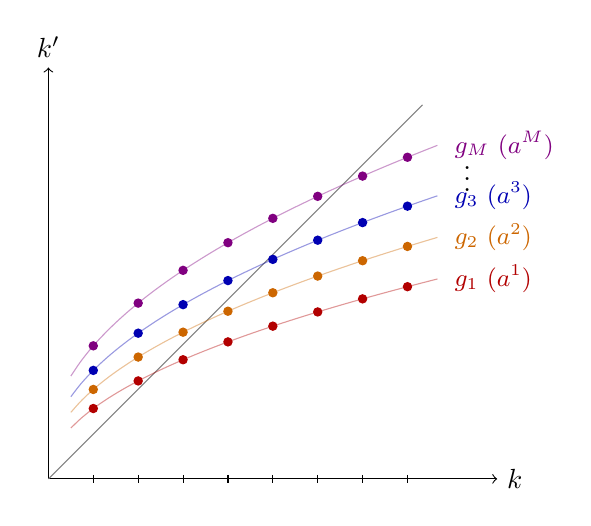
\begin{tikzpicture}[scale=0.95]
    \draw[->] (0,0) -- (6,0) node[right] {$k$};
    \draw[->] (0,0) -- (0,5.5) node[above] {$k'$};
    \draw[gray, thin] (0,0) -- (5,5);
    % Grid ticks
    \foreach \k in {0.6, 1.2, 1.8, 2.4, 3.0, 3.6, 4.2, 4.8} {
        \draw (\k, 1.5pt) -- (\k, -1.5pt);
    }
    % g for a^1 (lowest)
    \draw[red!70!black, thin, opacity=0.4] plot[smooth, domain=0.3:5.2, samples=40] (\x, {0.05+1.15*sqrt(\x)});
    \foreach \k in {0.6, 1.2, 1.8, 2.4, 3.0, 3.6, 4.2, 4.8} {
        \fill[red!70!black] (\k, {0.05+1.15*sqrt(\k)}) circle (1.8pt);
    }
    \node[red!70!black, right, font=\small] at (5.3, {0.05+1.15*sqrt(5.2)}) {$g_1\ (a^1)$};
    % g for a^2
    \draw[orange!80!black, thin, opacity=0.4] plot[smooth, domain=0.3:5.2, samples=40] (\x, {0.15+1.35*sqrt(\x)});
    \foreach \k in {0.6, 1.2, 1.8, 2.4, 3.0, 3.6, 4.2, 4.8} {
        \fill[orange!80!black] (\k, {0.15+1.35*sqrt(\k)}) circle (1.8pt);
    }
    \node[orange!80!black, right, font=\small] at (5.3, {0.15+1.35*sqrt(5.2)}) {$g_2\ (a^2)$};
    % g for a^3
    \draw[blue!70!black, thin, opacity=0.4] plot[smooth, domain=0.3:5.2, samples=40] (\x, {0.25+1.55*sqrt(\x)});
    \foreach \k in {0.6, 1.2, 1.8, 2.4, 3.0, 3.6, 4.2, 4.8} {
        \fill[blue!70!black] (\k, {0.25+1.55*sqrt(\k)}) circle (1.8pt);
    }
    \node[blue!70!black, right, font=\small] at (5.3, {0.25+1.55*sqrt(5.2)}) {$g_3\ (a^3)$};
    % g for a^M (highest)
    \draw[violet, thin, opacity=0.4] plot[smooth, domain=0.3:5.2, samples=40] (\x, {0.4+1.78*sqrt(\x)});
    \foreach \k in {0.6, 1.2, 1.8, 2.4, 3.0, 3.6, 4.2, 4.8} {
        \fill[violet] (\k, {0.4+1.78*sqrt(\k)}) circle (1.8pt);
    }
    \node[violet, right, font=\small] at (5.3, {0.4+1.78*sqrt(5.2)}) {$g_M\ (a^M)$};
    % Dots between a^3 and a^M
    \node at (5.6, {0.5*(0.25+1.55*sqrt(5.2) + 0.4+1.78*sqrt(5.2))}) {$\vdots$};
\end{tikzpicture}
\end{center}

\subsubsection*{Step 5: Simulate}

Given initial conditions $k_0$ and $a_0$, simulate $\{a_t\}_{t=0}^T$ from the Markov chain $\Pi$, then iterate:
$$
k_{t+1} = g(a_t, k_t), \qquad y_t = e^{a_t} f(k_t), \qquad I_t = k_{t+1} - (1-\delta)k_t, \qquad c_t = y_t - I_t.
$$
The simulated series $\{k_{t+1}, c_t, y_t, I_t\}$ can then be used to compute business cycle statistics and compare the model's predictions against the data.

\section{An RBC Model with Endogenous Labor}

The fixed-labor RBC model can match Facts 1 and 2 (investment volatility and pro-cyclical productivity), but it is silent on Fact 3 (cyclicality of total hours). To address all three facts simultaneously, we now extend the model to allow the planner to choose \textbf{labor supply} $L$ in addition to consumption and investment.

\subsection{The Planner's Problem}

Since labor $L$ is now a choice variable, we write the problem in aggregate terms $(C, K, L)$ rather than per-capita terms.\footnote{There are two reasons. First, a technical one: when $L$ varies over time, per-capita variables like $k_t = K_t/L_t$ have the endogenous choice $L_t$ in the denominator, making the transformation messy (though not impossible). Second, and more fundamentally: the whole point of introducing endogenous labor is to model the \textit{fluctuation of aggregate hours} $L$ and test whether it matches Fact 3. If we divided through by $L$ and worked in per-capita terms, the variable $L$ would be normalized away from the Bellman equation, and we would lose the ability to study its cyclical behavior. We need $L$ to appear explicitly as a choice variable.} The Bellman equation in aggregate terms is:
$$
\ba
V(a, K) &= \max_{C,\, L,\, K'} \left\{ u(C, L) + \beta\, \E{V(a', K') \mid a} \right\} \\
\text{s.t.} &\quad C + K' = e^a F(K, L) + (1-\delta)K, \\
&\quad C > 0, \quad K' \geq 0, \quad L \in (0, 1).
\ea
$$

The period utility $u(C, L)$ now depends on both consumption and labor. We assume:
$$
u_C > 0, \quad u_{CC} < 0, \quad u_L < 0, \quad u_{LL} < 0.
$$
The first pair says the agent likes consumption with diminishing marginal utility. The second pair says the agent dislikes working, and the marginal disutility of labor is \textit{increasing}: each additional hour of work is more painful than the last.

\subsection{Characterizing the Solution: Two Euler Equations}

We derive the optimality conditions in three steps: 
\begin{itemize}
    \item Take FOCs of the Bellman equation with respect to $C$, $L$, and $K'$; 
    \item Apply the envelope theorem;
    \item Substitute the envelope condition into the FOCs to eliminate the value function. This yields two Euler equations.
\end{itemize}

\subsubsection*{Inter-temporal Euler Equation $(EE_K)$}

The FOC with respect to $K'$ and the envelope condition together give:
\begin{equation}
u_C(C, L) = \beta\, \E{u_C(C', L') \Big( \underbrace{e^{a'} F_K(K', L')}_{\text{MPK}'} + 1 - \delta \Big) \,\middle|\, a}
\tag{$EE_K$}
\end{equation}

This is the standard consumption Euler equation: the marginal cost of saving one more unit today (left side: foregone marginal utility of consumption) equals the expected marginal benefit tomorrow (right side: the additional unit of capital earns the marginal product of capital $e^{a'}F_K(K',L')$ net of depreciation, valued at tomorrow's marginal utility).

\subsubsection*{Intra-temporal Euler Equation $(EE_L)$}

The FOC with respect to $L$ gives:
\begin{equation}
-u_L(C, L) = u_C(C, L) \cdot \underbrace{e^a F_L(K, L)}_{\text{MPL}}
\tag{$EE_L$}
\end{equation}

This is a \textbf{static} condition---it involves only time-$t$ variables. It says the marginal disutility of working one more hour (left side) must equal the marginal utility of the extra consumption that hour produces (right side: the marginal product of labor, converted to utility units by multiplying by $u_C$).\footnote{MPL $\equiv e^a F_L(K,L)$ is the \textit{marginal product of labor}: the additional output produced by one more unit of labor, holding capital fixed. MPK $\equiv e^a F_K(K,L)$ is the \textit{marginal product of capital}: the additional output from one more unit of capital, holding labor fixed. In a competitive equilibrium, MPL equals the real wage and MPK equals the rental rate of capital.}

\rmkb[]{
    Note that $(EE_K)$ is an \textit{inter-temporal} condition (linking $t$ and $t+1$), while $(EE_L)$ is an \textit{intra-temporal} condition (a within-period trade-off between leisure and consumption). Together with the resource constraint, they fully characterize the optimal allocation.
}

\subsection{Parameterization and the Frisch Elasticity}

To make the model quantitative, we adopt a standard parameterization that separates consumption utility from labor disutility:
$$
u(C, L) = \frac{C^{1-\sigma}}{1-\sigma} - B \frac{L^{1+\frac{1}{\nu}}}{1+\frac{1}{\nu}},
$$
where $\sigma > 0$ is the coefficient of relative risk aversion (governing the curvature of consumption utility), $B > 0$ scales the disutility of labor, and $\nu > 0$ is a parameter that controls the labor supply elasticity.

Under this specification, the partial derivatives are:
$$
u_C = C^{-\sigma}, \qquad u_L = -B L^{1/\nu}.
$$
Plugging into $(EE_L)$:
$$
B L^{1/\nu} = C^{-\sigma} \cdot \text{MPL},
$$
which, after rearranging, gives:
$$
L = \left(\frac{1}{B}\right)^\nu C^{-\sigma\nu} \cdot \text{MPL}^\nu.
$$
Taking logs:
$$
\ln L = \text{const.} - \sigma\nu \ln C + \nu \ln \text{MPL}.
$$

\defn{Frisch Elasticity of Labor Supply}{
    The \textbf{Frisch elasticity} measures the responsiveness of labor supply to changes in the wage (marginal product of labor), \textit{holding the marginal utility of wealth constant}:
    $$
    \text{Frisch Elasticity} \equiv \frac{\partial \ln L}{\partial \ln \text{MPL}} \bigg|_{u_C = \text{const.}} = \nu.
    $$
    A higher $\nu$ means that hours worked respond more strongly to changes in the wage. This elasticity is the key parameter governing how much labor fluctuates over the business cycle.
}

\rmkb[]{
    \begin{itemize}
        \item The condition $u_C = \text{const.}$ isolates the \textit{intertemporal substitution} channel. To see why, consider a worker deciding how many hours to work today vs.\ tomorrow. Suppose wages are temporarily high today but will return to normal tomorrow. The worker faces two competing effects:
        
        \textit{Substitution effect:} ``Wages are high today, so each hour of work buys more consumption. I should work more today and take leisure tomorrow.'' This effect increases current labor supply.
        
        \textit{Wealth effect:} ``I'm richer overall because of the high wage. Since I'm richer, I can afford more leisure.'' This effect decreases current labor supply.
        
        The Frisch elasticity captures \textit{only} the substitution effect by holding $u_C$ constant. Here is why this shuts down the wealth channel. When wages rise permanently, the agent is richer in a lifetime sense. A richer agent consumes more ($C$ rises), which means $u_C = C^{-\sigma}$ \textit{falls}. Looking back at the labor supply equation $\ln L = \text{const.} - \sigma\nu \ln C + \nu \ln \text{MPL}$, we see that higher $C$ (lower $u_C$) reduces $L$---this is precisely the wealth effect (``I'm richer, so I consume more leisure''). By holding $u_C$ constant, we freeze $C$ at its current level and ask: if only the wage changes but the agent's wealth position does not, how much does labor supply respond? This isolates the pure substitution motive. If the wage increase is truly temporary (as business cycle shocks are), the wealth effect is small (one good quarter barely changes lifetime income), so the Frisch elasticity is the relevant measure. If the wage increase were permanent, the wealth effect would be large, and the total (Marshallian) labor supply elasticity---which combines both effects---would be smaller than the Frisch elasticity.
        \item For any variable $x$, $\d \ln x = \d x / x$ is approximately the percentage change. So the Frisch elasticity $\nu = \partial \ln L / \partial \ln \text{MPL}$ is literally ``the percent change in hours worked per one percent change in the wage''---exactly the standard notion of elasticity from intermediate micro, applied to the specific context of labor supply. What makes it ``Frisch'' is the ceteris paribus condition: we hold the marginal utility of wealth fixed, which isolates the pure substitution effect of a wage change.
    \end{itemize}
}

\subsection{Discussion: The Frisch Elasticity Puzzle}

The model with endogenous labor faces a serious quantitative tension when we try to match all three business cycle facts simultaneously.

\subsubsection*{What the Model Needs}

Consider the labor market response to a positive productivity shock ($a$ increases). The shock raises the MPL, which shifts the labor demand curve outward from $L^D_L$ to $L^D_H$. How much equilibrium hours change depends on the slope of the labor supply curve, which is governed by the Frisch elasticity $\nu$.

\begin{center}
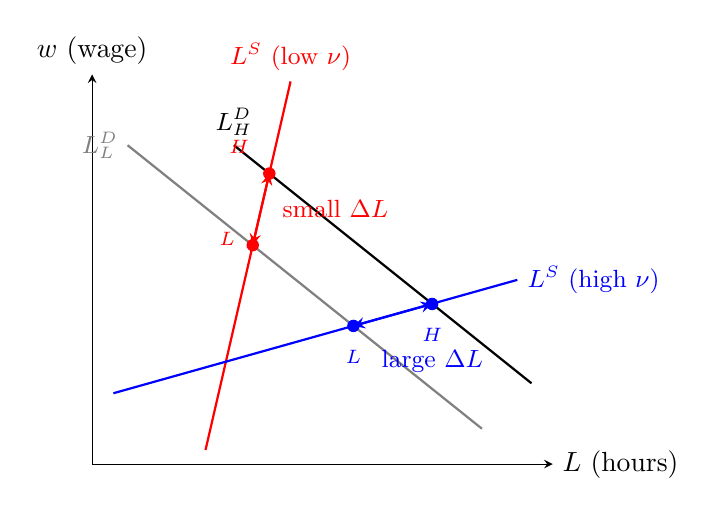
\begin{tikzpicture}[scale=0.9, >=stealth]
    % Axes
    \draw[->] (0,0) -- (6.5,0) node[right] {$L$ (hours)};
    \draw[->] (0,0) -- (0,5.5) node[above] {$w$ (wage)};
    
    % Labor demand L^D_L: from (0.5, 4.5) to (5.5, 0.5)
    % slope = (0.5 - 4.5)/(5.5 - 0.5) = -0.8
    % w = 4.5 - 0.8(L - 0.5) = 4.9 - 0.8 L
    \draw[thick, gray] (0.5,4.5) -- (5.5,0.5);
    \node[gray, font=\small, left] at (0.5,4.5) {$L^D_L$};
    
    % Labor demand L^D_H: shifted right by 1.5
    % from (2.0, 4.5) to (7.0, 0.5), but clip at 6.2
    % w = 4.5 - 0.8(L - 2.0) = 6.1 - 0.8 L
    \draw[thick, black] (2.0,4.5) -- (6.2,1.14);
    \node[black, font=\small, above] at (2.0,4.5) {$L^D_H$};
    
    % Labor supply steep (low nu): from (1.6, 0.2) to (2.8, 5.4)
    % slope = 5.2/1.2 = 4.333
    % w = 0.2 + 4.333(L - 1.6) = 4.333 L - 6.733
    \draw[thick, red] (1.6,0.2) -- (2.8,5.4) node[above, font=\small] {$L^S$ (low $\nu$)};
    
    % Intersection steep supply with L^D_L:
    % 4.333 L - 6.733 = 4.9 - 0.8 L => 5.133 L = 11.633 => L = 2.266, w = 3.087
    \fill[red] (2.266, 3.09) circle (2.5pt);
    \node[red, font=\scriptsize, above left] at (2.15, 2.95) {$L$};
    
    % Intersection steep supply with L^D_H:
    % 4.333 L - 6.733 = 6.1 - 0.8 L => 5.133 L = 12.833 => L = 2.500, w = 4.10
    \fill[red] (2.500, 4.10) circle (2.5pt);
    \node[red, font=\scriptsize, above left] at (2.35, 4.25) {$H$};
    
    \draw[<->, red, thick] (2.266, 3.09) -- (2.500, 4.10);
    \node[red, font=\scriptsize, right] at (2.55, 3.6) {\small small $\Delta L$};
    
    % Labor supply flat (high nu): from (0.3, 1.0) to (6.0, 2.6)
    % slope = 1.6/5.7 = 0.2807
    % w = 1.0 + 0.2807(L - 0.3) = 0.9158 + 0.2807 L
    \draw[thick, blue] (0.3,1.0) -- (6.0,2.6) node[right, font=\small] {$L^S$ (high $\nu$)};
    
    % Intersection flat supply with L^D_L:
    % 0.9158 + 0.2807 L = 4.9 - 0.8 L => 1.0807 L = 3.9842 => L = 3.687, w = 1.951
    \fill[blue] (3.687, 1.95) circle (2.5pt);
    \node[blue, font=\scriptsize, below] at (3.687, 1.75) {$L$};
    
    % Intersection flat supply with L^D_H:
    % 0.9158 + 0.2807 L = 6.1 - 0.8 L => 1.0807 L = 5.1842 => L = 4.797, w = 2.262
    \fill[blue] (4.797, 2.26) circle (2.5pt);
    \node[blue, font=\scriptsize, below] at (4.797, 2.06) {$H$};
    
    \draw[<->, blue, thick] (3.687, 1.95) -- (4.797, 2.26);
    \node[blue, font=\scriptsize, below] at (4.8, 1.75) {\small large $\Delta L$};
\end{tikzpicture}
\end{center}

As the diagram shows, a steep labor supply curve (low $\nu$, red) implies that the same demand shift produces only a small change in equilibrium hours---most of the adjustment shows up in wages. A flat supply curve (high $\nu$, blue) instead generates a large change in hours with only a modest wage response. 

To match \textbf{Fact 3} (total hours are as cyclical as output), the model needs the latter scenario: labor supply must be highly elastic. Quantitatively, matching both Fact 2 and Fact 3 simultaneously requires a Frisch elasticity of:
$$
\hat{\nu}_{\text{RBC}} > 4.
$$

\subsubsection*{What Micro Data Say}

The micro labor literature estimates the Frisch elasticity using individual-level data---measuring how much a given worker adjusts hours in response to temporary wage changes (e.g., overtime premia, tax holidays). The consensus from this literature is:
$$
\hat{\nu}_{\text{micro}} \ll 1, \quad \text{typically } 0.1 \text{--} 0.2.
$$
That is, individual workers barely adjust their hours when wages change temporarily. This is strikingly at odds with the $\hat{\nu}_{\text{RBC}} > 4$ required by the RBC model---a discrepancy of more than an order of magnitude.

\subsubsection*{Potential Resolutions}

There are two main avenues for reconciling the high macro elasticity with the low micro elasticity:

\textbf{1. Aggregation via the Extensive Margin.} Recall from Fact 3 that roughly 2/3 of the cyclical variation in total hours comes from the extensive margin (workers entering and leaving employment), not the intensive margin (hours per worker). Micro estimates of the Frisch elasticity capture only the \textit{intensive margin}---how much an already-employed worker adjusts hours. But at the macro level, what matters is the \textit{aggregate} response of total hours $\sum_i h_i$, which includes the extensive margin response of workers who move in and out of employment entirely. Even if each individual has a low intensive-margin elasticity, the aggregate elasticity can be much larger if the extensive margin is responsive. This partially closes the gap---but the extensive margin alone accounts for only about 1/3 of the discrepancy, so it is not a complete resolution.

\rmkb[Why the Extensive Margin Is Missed by Micro Estimates]{
    The logic is as follows. Micro studies estimate the Frisch elasticity by regressing an individual's hours on their wage, using workers who are \textit{continuously employed}. This captures the intensive margin: how an employed person adjusts hours at the margin. But during a recession, many workers do not reduce hours---they lose their jobs entirely (or during a boom, previously non-employed workers enter the labor force). These discrete 0-to-1 or 1-to-0 transitions constitute the extensive margin. Since a worker who exits employment has no ``hours vs.\ wage'' data point, the extensive margin response is invisible in micro panel regressions.
    
    At the aggregate level, total hours $= \text{(number of workers)} \times \text{(hours per worker)}$. The micro Frisch elasticity governs only the second term. Empirically, the first term is highly responsive to aggregate conditions: during the Great Recession, average hours per worker fell by only about 1\%, while the number of employed workers fell by roughly 6\%. This is not just a theoretical possibility---it is a well-documented pattern (see Fact 3: 2/3 of hours variation is extensive margin). Workers who remain employed show little change in their individual hours (consistent with $\hat{\nu}_{\text{micro}} \approx 0.1$--$0.2$), but the aggregate labor input swings dramatically because many workers transition between employment and non-employment. This is why the \textit{macro} Frisch elasticity (governing the response of total hours) can far exceed the \textit{micro} Frisch elasticity. However, accounting for this channel closes roughly 1/3 of the gap, leaving a substantial residual discrepancy.
}
\textbf{2. Non-competitive or Frictional Labor Markets.} The RBC model assumes a perfectly competitive, frictionless labor market in which workers are always on their labor supply curve. In particular, the wage always equals the MPL, and employment is determined by the intersection of supply and demand. This is what forces the model to need a high Frisch elasticity: the \textit{only} way to generate large hours fluctuations in a competitive market is to have a flat supply curve.

But real labor markets are not frictionless. Two important departures:

\begin{itemize}
    \item \textbf{Wage stickiness.} Suppose wages cannot adjust freely in the short run---they are ``sticky'' due to long-term contracts, social norms against wage cuts, or institutional constraints.
    
    Consider first a \textit{negative} productivity shock. The MPL falls below the prevailing wage $\bar{w}$. The firm now faces a choice: cut wages for all workers to match the new MPL, or lay off some workers while keeping the remaining workers' wages unchanged. In practice, firms overwhelmingly choose layoffs over across-the-board wage cuts.\footnote{This is a robust empirical finding. Bewley (1999) documents through extensive interviews that managers strongly resist nominal wage cuts, citing concerns about worker morale, effort, and retention.} Workers who keep their jobs face the same wage as before, so their individual labor supply barely changes---consistent with a low micro Frisch elasticity. The entire drop in aggregate hours comes from workers who are laid off (extensive margin), a discrete jump that has nothing to do with anyone sliding along a labor supply curve.
    
    The logic is symmetric in \textit{booms}. When a positive shock raises the MPL above $\bar{w}$, firms find it profitable to hire additional workers at the existing wage rather than raise wages for current employees. Each new hire generates surplus since MPL $> \bar{w}$. The result is a large increase in employment with little movement in wages or incumbent workers' hours. 
    
    In both directions, wage rigidity channels aggregate fluctuations into the extensive margin, generating large swings in total hours without requiring a high Frisch elasticity.
    
    \begin{center}
    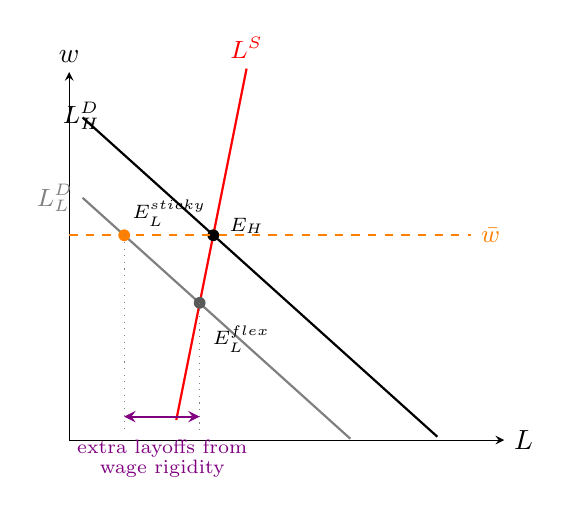
\begin{tikzpicture}[scale=0.85, >=stealth]
        \draw[->] (0,0) -- (6.5,0) node[right] {$L$};
        \draw[->] (0,0) -- (0,5.5) node[above] {$w$};
        
        % Labor supply (steep, true micro elasticity)
        % w = 5(L - 1.6) + 0.3 = 5L - 7.7
        \draw[thick, red] (1.6, 0.3) -- (2.65, 5.55);
        \node[red, font=\small, above] at (2.65, 5.55) {$L^S$};
        
        % Demand good: w = -0.9L + 5.0
        \draw[thick, black] (0.2, 4.82) -- (5.5, 0.05);
        \node[black, font=\small, above left] at (0.6, 4.5) {$L^D_H$};
        
        % Demand bad: w = -0.9L + 3.8
        \draw[thick, gray] (0.2, 3.62) -- (4.2, 0.02);
        \node[gray, font=\small, left] at (0.2, 3.62) {$L^D_L$};
        
        % Good-state equilibrium: 5L - 7.7 = -0.9L + 5.0 => 5.9L = 12.7 => L = 2.153, w = 3.06
        \fill[black] (2.153, 3.06) circle (2.5pt);
        \node[font=\scriptsize, right] at (2.25, 3.2) {$E_H$};
        
        % Sticky wage at good-state level
        \draw[dashed, thick, orange] (0, 3.06) -- (6, 3.06) node[right, font=\small] {$\bar{w}$};
        
        % Flexible-wage bad-state eq: 5L - 7.7 = -0.9L + 3.8 => 5.9L = 11.5 => L = 1.949, w = 2.046
        \fill[gray!70!black] (1.949, 2.05) circle (2.5pt);
        \node[font=\scriptsize, below right] at (2.0, 1.85) {$E_L^{\text{flex}}$};
        
        % Sticky-wage bad-state: on demand_L at w = 3.06
        % -0.9L + 3.8 = 3.06 => L = 0.822
        \fill[orange] (0.822, 3.06) circle (2.5pt);
        \node[font=\scriptsize, above right] at (0.8, 3.05) {$E_L^{\text{sticky}}$};
        
        % Arrow showing excess layoffs
        \draw[dotted, gray] (0.822, 3.06) -- (0.822, 0.15);
        \draw[dotted, gray] (1.949, 2.05) -- (1.949, 0.15);
        \draw[<->, thick, violet] (0.822, 0.35) -- (1.949, 0.35);
        \node[violet, font=\scriptsize, below] at (1.39, 0.15) {extra layoffs from};
        \node[violet, font=\scriptsize, below] at (1.39, -0.15) {wage rigidity};
    \end{tikzpicture}
    \end{center}
    
    Under flexible wages, a negative shock moves the equilibrium from $E_H$ to $E_L^{\text{flex}}$: both wages and hours fall modestly. Under sticky wages, the wage stays at $\bar{w}$, so the firm slides along its demand curve to $E_L^{\text{sticky}}$, laying off all workers whose MPL falls below the rigid wage. The violet arrow marks the additional employment loss caused purely by wage rigidity.

\rmkb[A Caveat on Identification]{
    An important limitation of the wage stickiness explanation is that it is difficult to test directly. If wages truly do not move, then we never observe the counterfactual flexible-wage equilibrium, and we cannot identify the slope of the labor supply curve from aggregate data. The observed variation in hours is driven entirely by demand shifts along a rigid wage, so the data are equally consistent with \textit{any} value of the micro Frisch elasticity. In this sense, sticky wages can ``explain'' any pattern of hours fluctuations, making the theory hard to falsify. However, there is independent micro-level evidence that wages are indeed sticky (e.g., Bewley, 1999; Barattieri, Basu, and Gottschalk, 2014), which lends external validity to this channel.
}
    
    \item \textbf{Monopsony power.} In a perfectly competitive labor market, firms are price-takers: they hire until MPL $= w$. Under monopsony, a single firm (or a firm with market power) faces an upward-sloping labor supply curve---to hire more workers, it must raise the wage for \textit{all} workers. This creates a wedge: the \textit{marginal cost of labor} (MCL) exceeds the wage, because hiring one more worker raises the wage bill for all existing workers.
    
    \begin{center}
    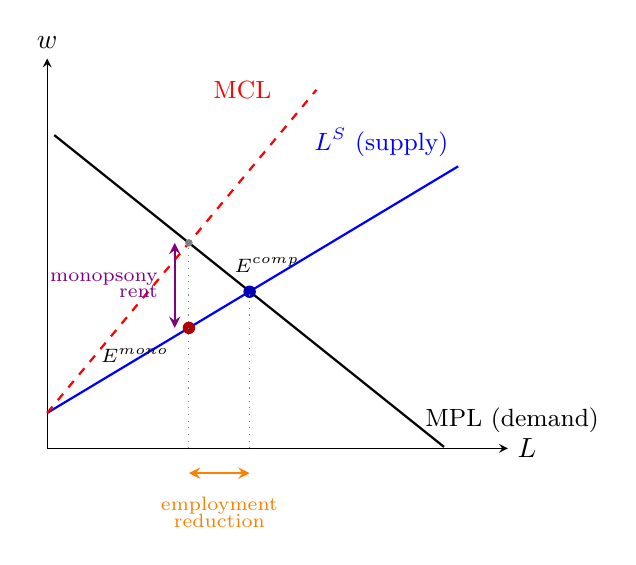
\begin{tikzpicture}[scale=0.9, >=stealth]
        \draw[->] (0,0) -- (6.5,0) node[right] {$L$};
        \draw[->] (0,0) -- (0,5.5) node[above] {$w$};
        
        % Labor supply: w = 0.5 + 0.6L
        \draw[thick, blue] (0, 0.5) -- (5.8, 3.98);
        \node[blue, font=\small, above left] at (5.8, 3.98) {$L^S$ (supply)};
        
        % MCL: w = 0.5 + 1.2L (twice the slope of supply)
        \draw[thick, red, dashed] (0, 0.5) -- (3.8, 5.06);
        \node[red, font=\small, left] at (3.3, 5.06) {MCL};
        
        % MPL (demand): w = 4.5 - 0.8L
        \draw[thick, black] (0.1, 4.42) -- (5.6, 0.02);
        \node[black, font=\small, right] at (5.2, 0.4) {MPL (demand)};
        
        % Competitive eq: supply = demand
        % 0.5 + 0.6L = 4.5 - 0.8L => 1.4L = 4 => L = 2.857, w = 2.214
        \fill[blue!70!black] (2.857, 2.21) circle (2.5pt);
        \node[font=\scriptsize, above] at (3.1, 2.35) {$E^{\text{comp}}$};
        
        % Monopsony eq: MCL = MPL
        % 0.5 + 1.2L = 4.5 - 0.8L => 2L = 4 => L = 2.0
        % MCL at L=2: 0.5 + 2.4 = 2.9
        % Wage paid (on supply curve at L=2): 0.5 + 1.2 = 1.7
        \fill[red!70!black] (2.0, 1.7) circle (2.5pt);
        \node[font=\scriptsize, below left] at (1.85, 1.55) {$E^{\text{mono}}$};
        
        % Dotted lines from monopsony point
        \draw[dotted, gray] (2.0, 0) -- (2.0, 2.9);
        \draw[dotted, gray] (2.857, 0) -- (2.857, 2.21);
        
        % MCL point (for markup reference)
        \fill[gray] (2.0, 2.9) circle (1.5pt);
        
        % Markup annotation (between wage paid and MPL at L=2)
        % MPL at L=2: 4.5 - 1.6 = 2.9
        \draw[<->, thick, violet] (1.8, 1.7) -- (1.8, 2.9);
        \node[violet, font=\scriptsize, left, align=right] at (1.7, 2.3) {monopsony\\[-2pt]rent};
        
        % Employment gap annotation
        \draw[<->, thick, orange] (2.0, -0.35) -- (2.857, -0.35);
        \node[orange, font=\scriptsize, below, align=center] at (2.43, -0.55) {employment\\[-2pt]reduction};
    \end{tikzpicture}
    \end{center}
    
    In a competitive market, firms hire until MPL $= w$, reaching $E^{\text{comp}}$. A monopsonist recognizes that hiring an extra worker raises the wage for \textit{all} workers, so the marginal cost of labor (MCL, red dashed) lies above the supply curve. The monopsonist hires where MCL $=$ MPL, reaching $E^{\text{mono}}$ with fewer workers (orange gap) paid a lower wage. The violet arrow shows the \textbf{monopsony rent}: the wedge between what the last worker produces and what the firm pays. When productivity shifts, the monopsonist adjusts employment along the MCL $=$ MPL margin---governed by the firm's market power, not by workers' labor supply elasticity. This breaks the tight link between the Frisch elasticity and aggregate hours fluctuations.
\end{itemize}

These insights motivate \textbf{New Keynesian} models, which embed nominal rigidities (sticky prices, sticky wages) into the RBC framework. In such models, aggregate hours can fluctuate substantially over the business cycle---driven by demand-side forces and wage rigidity---without requiring an implausibly high Frisch elasticity. The elasticity $\nu$ remains a property of individual preferences (a ``result'' of the utility function parameterization), but in a New Keynesian world, the \textit{equilibrium response of hours} is no longer pinned down by $\nu$ alone---it also depends on the degree of wage stickiness and market power.

